\documentclass{article}


\usepackage{PRIMEarxiv}

\usepackage[utf8]{inputenc} % allow utf-8 input
\usepackage[T1]{fontenc}    % use 8-bit T1 fonts
\usepackage{hyperref}       % hyperlinks
\usepackage{url}            % simple URL typesetting
\usepackage{booktabs}       % professional-quality tables
\usepackage{amsfonts}       % blackboard math symbols
\usepackage{nicefrac}       % compact symbols for 1/2, etc.
\usepackage{microtype}      % microtypography
\usepackage{lipsum}
\usepackage{enumitem}
\usepackage{amsmath}
\usepackage{fancyhdr}       % header
\usepackage{graphicx}       % graphics
\graphicspath{{media/}}     % organize your images and other figures under media/ folder
\usepackage[export]{adjustbox}   % JS add for logo
\usepackage{natbib}              % JS add for citep()
\usepackage[english]{babel}
% \bibliographystyle{abbrvnat}  
% \bibliographystyle{unsrt}  
% \bibliographystyle{plain}
\bibliographystyle{unsrtnat}
\setcitestyle{authoryear, open={((},close={)}}

% \immediate\write18{cp `kpsewhich plain.bst` .}

\usepackage{caption}
\captionsetup[table]{skip=8pt}

\usepackage{lastpage}
%Header
% \fancypagestyle{firstpage}   %% from 
%% https://stackoverflow.com/questions/54736891/
% {
%     \fancyhead[L]{JBDAI Vol. XX No. X, pp. 1-XX/ 2021}    
%     \fancyhead[R]{ 
\includegraphics[width=4cm]{JBDAI.png}}
% }
% \thispagestyle{firstpage}
\pagestyle{fancy}
\thispagestyle{plain}


% Update your Headers here
\rhead{ \textit{ JBDAI Vol. 04 No. 1, pp. 1-n/ 2026}} 
% \fancyhead[LO]{}
% \fancyhead[RE]{Firstauthor and Secondauthor} % Firstauthor et al. if more than 2 - must use \documentclass[twoside]{article}



  
%% Title
\title{Benchmarking Open Source Vector Databases
%%%% Cite as
%%%% Update your official citation here when published 
% \thanks{\textit{\underline{Citation}}: 
% \textbf{Authors. Title. Pages.... DOI:000000/11111.}} 
}

\author{
  Jeet Patel \\
  M.S. in Computer Science \\
  Kwaai AI Lab, USA\\
  \texttt{jeetpt1405@gmail.com} \\
  %% examples of more authors
   \And
  Akshaya Dol \\
  M.S. in Computer Science \\  
  Kwaai AI Lab, USA \\
  \texttt{dolakshaya1995@gmail.com} \\
   \And
     Arun Chand \\
  MBA Business Analytics \\
  Kwaai AI Lab, USA \\
  \texttt{chandarun12@gmail.com} \\
   \And
  Selim Soufargi \\
  Ph.D. Data Science \\
  Kwaai AI Lab, USA \\
  \texttt{slim.s1988s@gmail.com} \\
   \And
  Sulimon Sattari \\
  PhD, Physics \\
  Kwaai AI Lab, USA \\
  \texttt{sulimon@kwaai.ai} \\
   \And
  Maira Khwaja \\
  B.Sc Biology \\
  Kwaai AI Lab, USA \\
  \texttt{maira@kwaai.ai} \\
   \And
  Reza Rassool \\
  Physics, King's College London;
  Affiliate Professor, University of Washington \\
  Kwaai AI Lab, USA \\
  \texttt{reza@kwaai.ai} \\
  %% \AND
  %% Coauthor \\
  %% Affiliation \\
  %% Address \\
  %% \texttt{email} \\
  %% \And
  %% Coauthor \\
  %% Affiliation \\
  %% Address \\
  %% \texttt{email} \\
  %% \And
  %% Coauthor \\
  %% Affiliation \\
  %% Address \\
  %% \texttt{email} \\
}

\begin{document}
% \begin{figure}
\begin{figure}
    
\includegraphics[width=0.4\textwidth, center]{JBDAI.png}
    \captionsetup{labelformat=empty}
    \caption{WWW.JBDAI.ORG}
    \caption{ISSN: xy xy xyy }   % To be assigned by JBDAI
    \caption{JBDAI Vol. 04 No. X, XXXX 2026   \hspace{1 cm}   DOI:10.54116 XXXX} % To be assigned by JBDAI
\end{figure}

% \begin{center}
% \begin{tabular}{ccc}

% DOI:10.3390/info11060314 &   & Received: 28 April 2020; Published: 11 June 2020 \\
% \end{tabular}
% \end{center}
% \caption{JBDAI Vol. XX No. X, pp. 1-XX/Forthcoming/ 2026}
% Early View / Accepted / Forthcoming
% \end{figure}
\maketitle

\begin{abstract}
Vector databases are a critical component of modern RAG systems, yet their scale performance characteristics are not sufficiently characterized. This paper evaluates the scalability, latency, throughput, and operational stability of seven widely used production vector databases such as FAISS, Chroma, Qdrant, Weaviate, Milvus, OpenSearch, and PGVector-across corpus sizes ranging from 175 to 2.2 million vector chunks, to provide practical guidance for system selection under real-world constraints.

We conducted a controlled benchmarking study using $N = 10$ independent trials per configuration. Query latency, throughput, ingestion performance, retrieval quality, and resource utilization are measured under consistent hardware, workload, and indexing settings. All databases are evaluated using identical embeddings and Top-$k$ retrieval parameters, with cold-start conditions enforced to eliminate cross-run caching effects. Variability is quantified using standard deviation and coefficient of variation to assess performance stability. Statistical outliers identified using modified Z-score methodology (threshold: |Z| > 3.5) are removed to distinguish transient cold-start behavior from steady-state performance.

The results reveal distinct performance regimes across systems and a critical cold-start phenomenon. Chroma exhibits near-constant-time query behavior (α = 0.02), achieving a latency of 7.7-8.4 ms and supporting up to 141 queries per second at medium scale. Chroma achieves exceptional consistency (CV = 2.3\% after removing 2 cold-start outliers, 8.8× improvement over raw variance) . PGVector with HNSW indexing achieves sub-10 ms latency and more than 100 queries per second at the 50k scale, outperforming all dedicated vector databases except Chroma. FAISS demonstrates strong sub-linear scaling ($\alpha = 0.48$) up to 2.2 million chunks with low variability (CV = 2.5\%). We further quantify an HNSW warm-up effect, observing latency reductions of up to 74\% as corpus size increases from 1k to 50k chunks. Most significantly, N=10 sampling with outlier removal reveals dramatic improvements in ingestion consistency: Qdrant CV 123\% → 1.0\% (122× improvement), Weaviate 107\% → 0.8\% (133× improvement), OpenSearch 93\% → 0.4\% (232× improvement). Resource analysis shows similar memory footprints (12-16 GB) across systems. Together, these findings clarify scalability limits, performance trade-offs, and the critical role of cold-start transient detection in vector database benchmarking.
\end{abstract}

\keywords{Vector databases \and Performance benchmarking \and Retrieval‑Augmented Generation (RAG) \and HNSW (Hierarchical Navigable Small World) \and Scalability analysis \and Query latency \& throughput \and Outlier detection \and Cold-start phenomena} 
\section{Introduction}
Vector databases have rapidly emerged as core infrastructure for modern AI systems~\cite{xie2023brief,jing2025large}. Applications such as retrieval-augmented generation (RAG)~\cite{lewis2020rag}, semantic search, recommendation systems, and production machine learning pipelines increasingly depend on efficient and predictable nearest-neighbor retrieval\cite{csakar2025maximizing}. Despite their growing importance, practitioners face significant uncertainty when selecting an appropriate vector database. Key system characteristics - including query latency, throughput, ingestion cost, consistency, persistence guarantees, and memory behavior - vary widely across implementations and deployment scales.

Existing benchmarking studies often evaluate relatively small corpora (typically fewer than 100k vectors), rely on single experimental runs without statistical
validation, and omit detailed analysis of resource utilization and performance variance. Consequently, critical questions surrounding scalability, reliability,
and production readiness remain insufficiently explored, particularly for deployments operating at million-scale corpus sizes. While tools such as ANN-Benchmarks and VectorDBBench have contributed to the evaluation of ANN algorithms and vector databases, they primarily emphasize retrieval accuracy and indexing performance. In contrast, our study extends this body of work by incorporating repeated trials ($N=10$), modified elimination of outliers of the Z-score, and systematic analysis of cold-start behavior and resource dynamics on scales up to 2.2 million vector factors essential for real-world deployment and
operational consistency.

This study directly addresses these limitations and expands the state of the art in three fundamental ways:
First, we perform our benchmarking analysis across four orders of magnitude from 175 to 2.2 million chunks extending prior work that maxes out at 100k vectors. This validates scaling behavior at production scales where single-node memory constraints, HNSW graph maturation effects, and performance degradation become critical to deployment decisions.
Second, we enforce a rigorous $N=10$ independent experimental protocol with complete database re-initialization per run, eliminating cross-run caching effects and capturing true run-to-run variability. We employ modified Z-score outlier detection to distinguish transient cold-start behavior from steady-state performance, quantifying consistency via coefficient of variation (CV). This extended sampling reveals that apparent "poor consistency" reflects database initialization overhead rather than algorithmic instability.
We provide significant reproducibility through publicly released code, configurations, and raw data.
Third, we conduct novel operational analyses, absent from prior benchmarks: characterization of HNSW "warm-up" effects (up to 74\% latency reduction from 1k to 50k chunks due to graph maturation), identification of retrieval quality paradoxes (U-shaped quality curves across scales), and measurement of the cold-start phenomenon (dramatic CV improvements after outlier removal: Qdrant 122×, Weaviate 133×, OpenSearch 232×). These insights directly inform deployment decisions beyond raw throughput metrics.

\textbf{Index Structure Context: HNSW and Flat Indexes.} A critical architectural distinction underlies vector database performance: 
the choice between approximate nearest neighbor (ANN) graph-based indexes and exact flat indexes. \textit{Hierarchical Navigable Small World 
(HNSW)} is a state-of-the-art ANN algorithm that constructs a multi-layered proximity graph over vector space, enabling logarithmic-time 
nearest neighbor search ($O(\log n)$ complexity) at the cost of 2-3× memory overhead and approximate recall. HNSW dominates production 
deployments for latency-sensitive applications at medium scales (10k-500k vectors). In contrast, \textit{flat indexes} (e.g., FAISS's 
IndexFlatIP) perform exhaustive linear search ($O(n)$ theoretical complexity) but achieve sub-linear practical performance ($\alpha \approx 0.48$) 
through SIMD vectorization and offer 100\% exact recall. The trade-off between these index structures-and how they scale with corpus 
size, available memory, and consistency requirements is fundamental to selecting an appropriate vector database for production deployments.

This work seeks to address the following research questions:
\begin{enumerate}
    \item \textbf{RQ1 (Scalability):} How do production vector databases scale from hundreds to millions of vector chunks with respect to query latency and throughput?    
    \item \textbf{RQ2 (Consistency and Reliability):} What is the run-to-run variance in ingestion and query workloads, and how does this variability impact service-level agreement (SLA) planning and total cost of ownership (TCO)?    
    \item \textbf{RQ3 (Resource Efficiency):} What are the CPU and memory footprints during query and ingestion workloads across scales, and how do these resource constraints limit single-node deployments?    
    \item \textbf{RQ4 (Architectural Trade-offs and Quality):} How do index structures and system architectures (e.g., flat vs.\ HNSW, embedded vs.\ client-server) affect performance, retrieval quality, and practical deployment decisions?
\end{enumerate}
This study benchmarks seven vector database systems: FAISS \cite{faiss_}, Chroma \cite{chromadb}, Qdrant \cite{qdrant}, Weaviate \cite{weaviate}, Milvus \cite{milvus}, OpenSearch \cite{opensearch}, and PGVector \cite{pgvector} across nine corpus sizes ranging from 175 to 2.2 million chunks. All experiments follow a reproducible statistical protocol with $N = 10$ independent runs per configuration. We employ sentence-transformer embeddings of 384 dimensions with a fixed chunking strategy of 512 characters and a 50-character overlap.

We measure median query latency (P50), query throughput (QPS), ingestion time, and resource utilization, sampling CPU and memory usage at a frequency of 1~Hz. Each experimental run uses a fresh database initialization to capture true run-to-run variability. Statistical outliers identified using modified Z-score methodology (threshold: |Z| > 3.5) are removed prior to aggregate statistics. All scripts, configurations, and raw experimental data are publicly available \cite{kwaai2025benchmark} to support reproducibility.
\subsection{Related Work}
\label{sec:related_work}

Benchmarking vector search systems has received increasing attention, as vector
databases have become core infrastructure for retrieval-augmented generation
(RAG), semantic search, and recommendation systems. Prior work can be broadly
classified into algorithm-level benchmarks, system-level database benchmarks,
cloud vendor evaluations, and foundational vector search studies.

\paragraph{Algorithm-Level Benchmarks.}
ANN-Benchmarks \cite{aumuller2020annbenchmarks} established a community standard
for evaluating approximate nearest neighbor (ANN) algorithms such as HNSW, IVF,
and PQ on standardized datasets. These benchmarks provide valuable insight
into algorithmic trade-offs between recall, latency, and memory usage.
However, they focus exclusively on algorithm implementations rather than
production-ready database systems and do not account for persistence,
concurrency, ingestion pipelines, or operational overheads.

Foundational ANN research includes HNSW \cite{malkov2018hnsw}, FAISS
\cite{johnson2019faiss}, ScaNN \cite{guo2020scann}, and DiskANN
\cite{jayaram2019diskann}, which explore graph-based and scalable quantization
approaches for high-dimensional vector search. Although these studies advance
algorithmic efficiency, they do not address end-to-end system behavior under
realistic deployment constraints.

\paragraph{System-Level Vector Database Benchmarks.}
VectorDBBench \cite{zilliz2024vectordbbench} represents one of the first
industry-led efforts to benchmark multiple vector databases, including Milvus
and related systems. Although it provides useful comparative information, it relies
primarily on single-run measurements ($N=1$) without statistical validation or
outlier analysis, limiting its ability to distinguish steady-state performance
from transient cold-start effects. In addition, its scale range evaluated is
narrower than that required for many production deployments.

\paragraph{Cloud Vendor Evaluations.}
Several cloud providers have published performance studies of proprietary vector
search services, including Pinecone \cite{pinecone2023benchmark}, AWS OpenSearch
\cite{awsopensearch2023}, and Azure Cognitive Search
\cite{azurevectorsearch2023}. These evaluations focus on managed, closed-source
platforms and often lack reproducibility due to undisclosed configurations,
proprietary optimizations, and opaque workload assumptions.

\paragraph{Positioning of This Work.}
Our study complements and extends previous benchmarks by focusing on
\emph{system-level performance of open-source production databases} under a
statistically rigorous experimental protocol. Unlike ANN-Benchmarks, we evaluate
complete database systems rather than isolated algorithms. In contrast to
VectorDBBench and cloud vendor studies, we employ $N=10$ independent runs per
configuration with modified Z-score outlier detection to separate cold-start
transients from steady-state behavior.

Table~\ref{tab:related_work_comparison} summarizes how this work compares with existing benchmarks. Specifically, this work contributes:
(i) the first statistically validated ($N=10$) benchmark across seven production
vector databases,
(ii) a broader evaluated scale range (175 to 2.2 million vectors),
(iii) rigorous outlier detection and consistency analysis,
(iv) comprehensive CPU and memory utilization measurements, and
(v) novel empirical characterization of HNSW warm-up effects and retrieval
quality dynamics across scale.


\begin{table}[t]
\centering
\small
\caption{Comparison with Existing Vector Search Benchmarks}
\begin{tabular}{lcccc}
\toprule
\textbf{Benchmark} & \textbf{Scale} & \textbf{Runs} & \textbf{Databases} & \textbf{Resource Analysis} \\
\midrule
ANN-Benchmarks & Algorithm-level & 1 & Algorithms & No \\
VectorDBBench & 100k-10M & 1 & 5 & Limited \\
Cloud Vendor Studies & Variable & 1 & Proprietary & No \\
\textbf{This Work} & 175-2.2M & \textbf{10} & \textbf{7} & \textbf{Yes} \\
\bottomrule
\end{tabular}
\label{tab:related_work_comparison}
\end{table}

\subsection{Key Contributions}
\begin{itemize}
    \item A publicly available benchmark suite \cite{kwaai2025benchmark} and a dataset that spans four orders of magnitude in corpus size with $N=10$ statistical validation and rigorous outlier detection using modified Z-score methodology.
    \item We construct a quantitative taxonomy that maps seven production vector databases to practical deployment scenarios, including latency-critical real-time RAG, large-scale workloads, and enterprise feature requirements (Section~\ref{sec:use_cases}).
    \item We characterize a behavior in HNSW-indexed systems that, to the authors' knowledge, has not been documented before in the literature at the time of this study, where query latency improves by up to 74\% as corpus size increases from 1k to 50k chunks due to graph maturation effects (Section~\ref{sec:hnsw_warmup}).
    \item We identify a counterintuitive U-shaped retrieval quality trend, with the lowest quality at approximately 1k chunks and a subsequent improvement of 27.5\% by 50k chunks, followed by saturation beyond 250-500k chunks (Section~\ref{sec:quality_paradox}).
    \item We demonstrate a critical cold-start phenomenon: N=10 sampling reveals that apparent poor consistency reflects initialization transients, not algorithmic instability. Multi-pass outlier cleaning shows dramatic improvements: Qdrant 123\% → 1.0\% CV (122× improvement), Weaviate 107\% → 0.8\% (133× improvement), OpenSearch 93\% → 0.4\% (232× improvement) (Section~\ref{sec:ingestion_consistency}).
    \item We establish memory-bound scaling ceilings for vector databases, showing that HNSW-based systems saturate at approximately 1-2M chunks under 16~GB RAM due to graph overhead, while flat indexes such as FAISS scale substantially further under identical hardware constraints (Section~\ref{sec:deployment_guidance}).    
\end{itemize}

\subsection{Organization of the Paper}
The paper is organized as follows. Section~\ref{sec: methods} describes the experimental methodology, including corpus preparation, the $N = 10$ statistical evaluation protocol, query and ingestion benchmarks, resource monitoring and data analysis methods. Section~\ref{sec: results} presents the experimental results, covering query latency scaling, throughput behavior, ingestion performance, resource utilization and retrieval quality. Section~\ref{sec: discussion} discusses architectural insights, system-level trade-offs and practical deployment implications derived from the results. Section~\ref{sec: conclusion} concludes the paper by summarizing key findings and performance implications. Section~\ref{sec:limitations} outlines limitations including sample size variation and scale restrictions. Section~\ref{sec: future} outlines directions for future work, including distributed scaling, GPU acceleration, hybrid retrieval workloads and expanded quality evaluation metrics.

\subsection{Multi-Database Scaling Performance Comparison}
\setcounter{figure}{0}
\begin{figure}[h!]
    \centering
    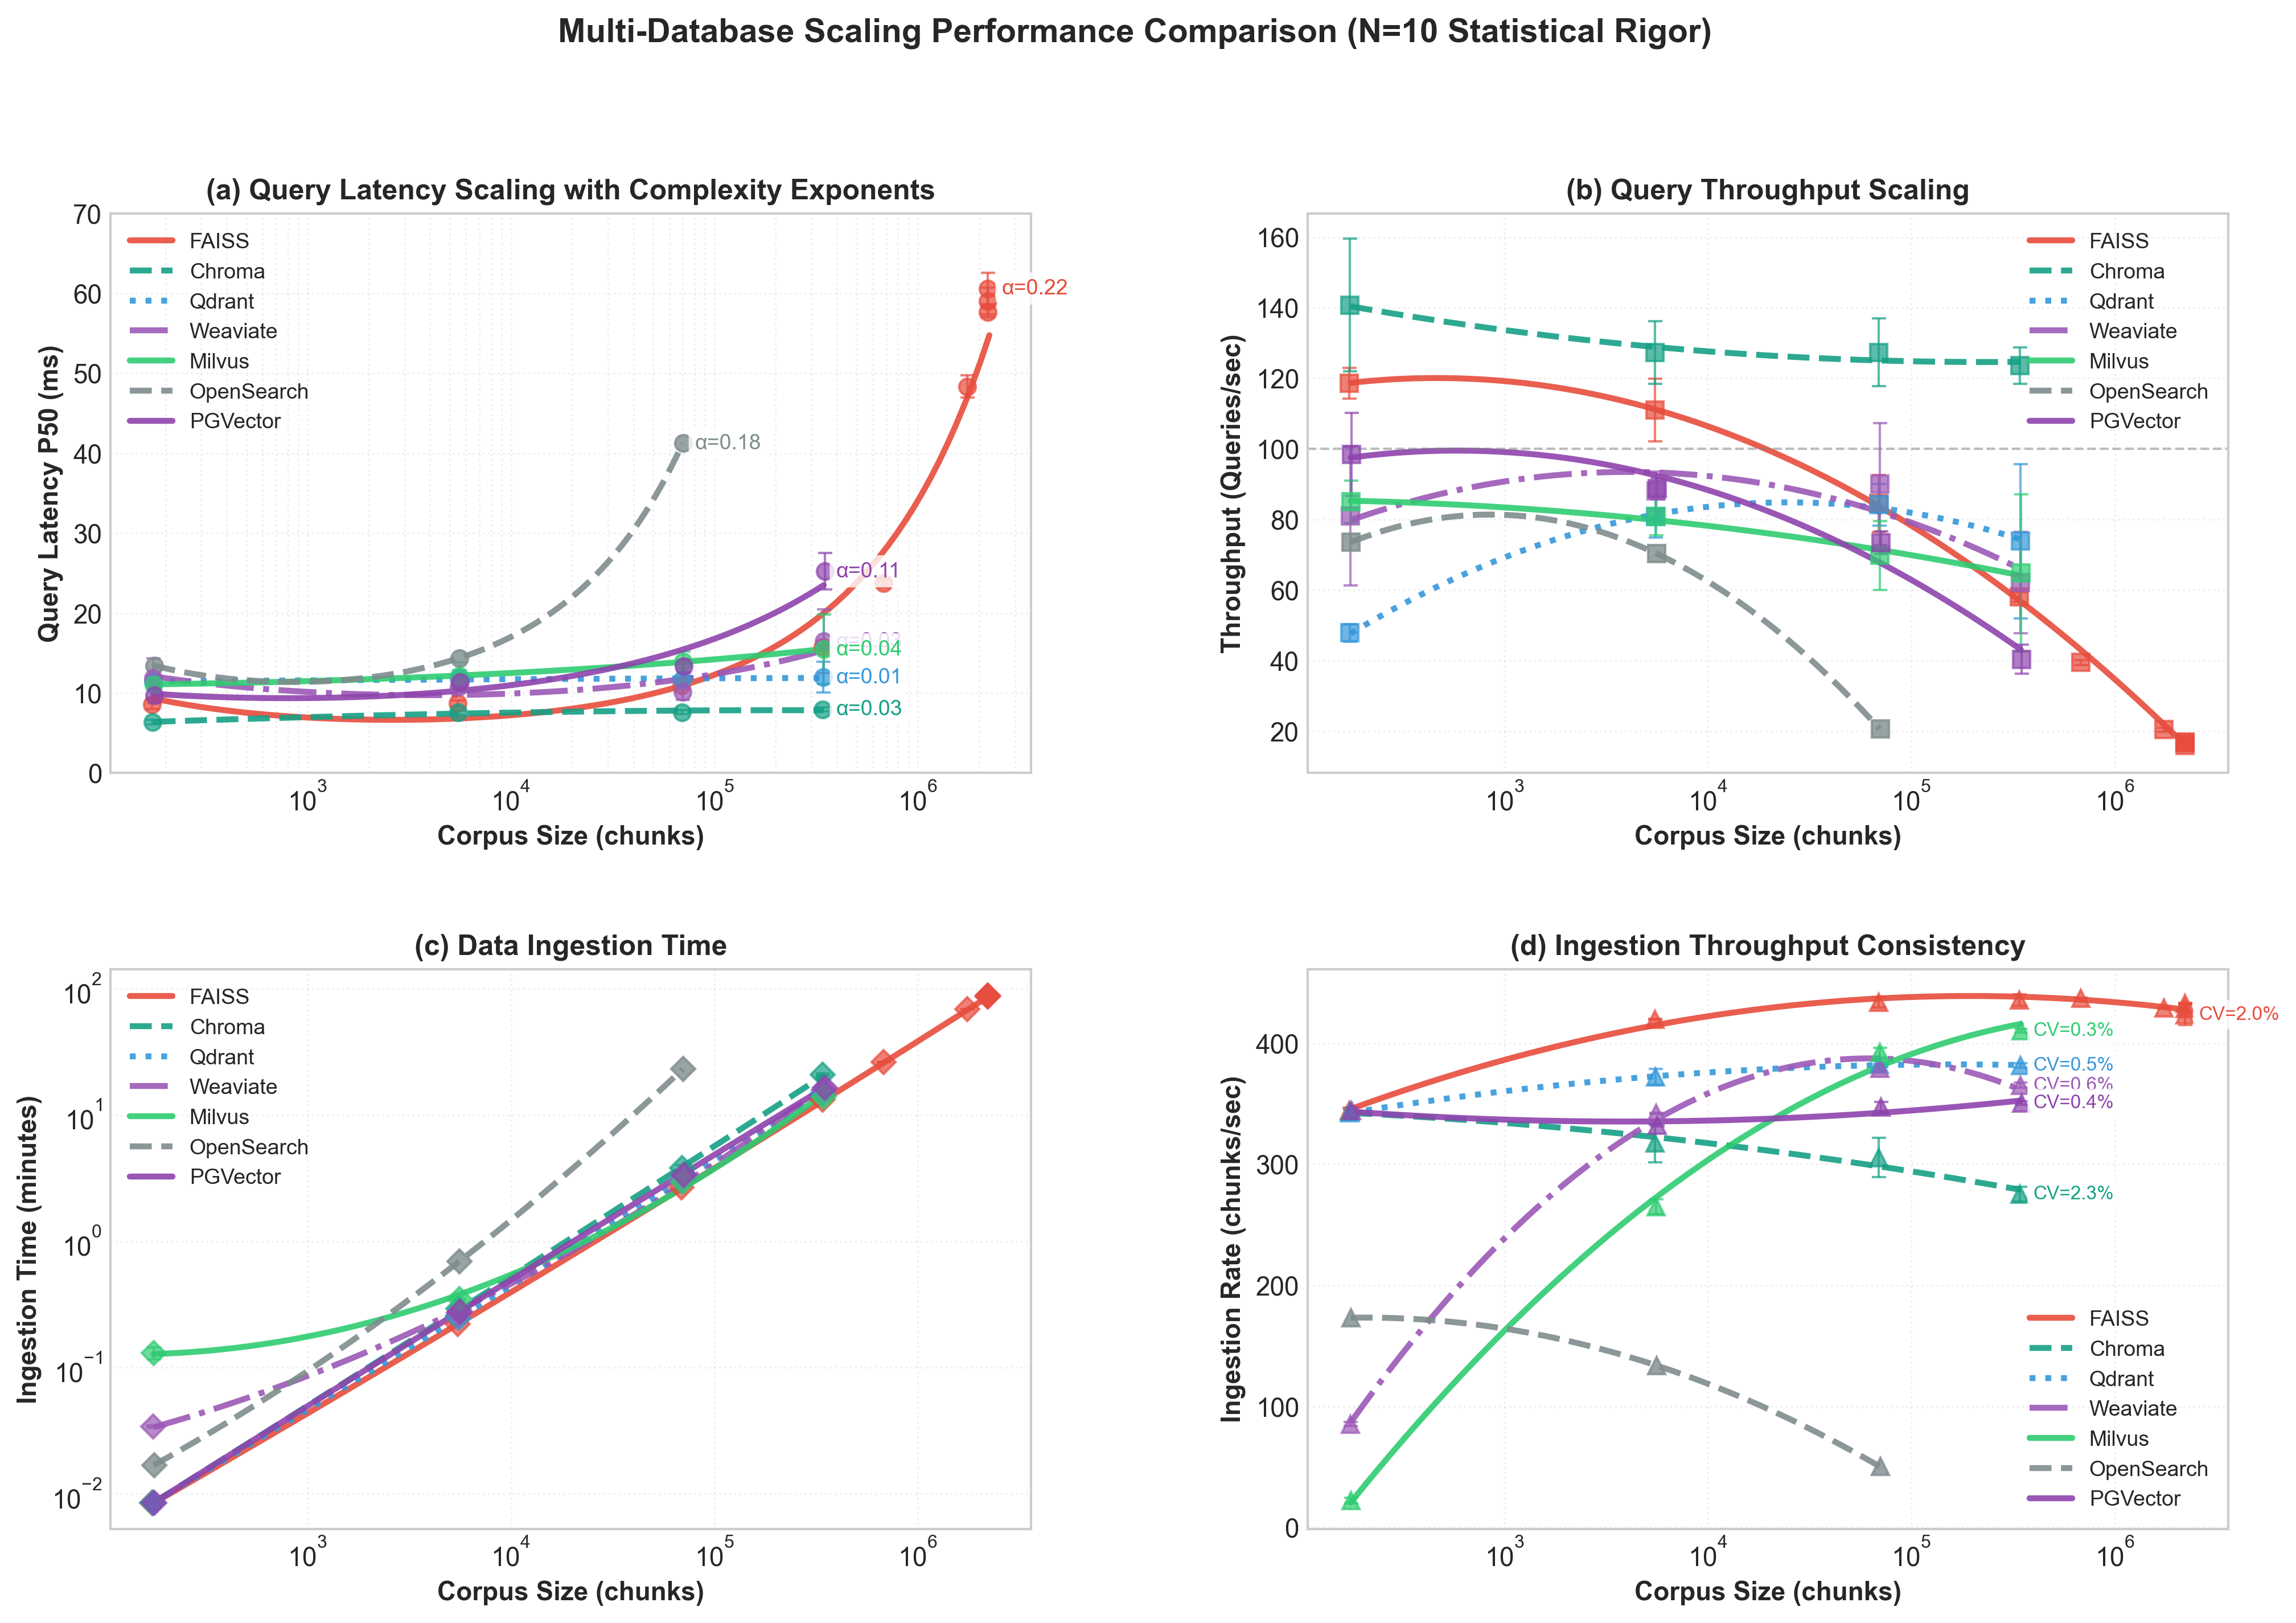
\includegraphics[width=1 \textwidth]{Multi-Database Scaling Performance Comparison.png}
    \caption{Multi-Database Scaling Performance Comparison (N=10, outliers removed)}
    \label{fig:Multi-Database Scaling Performance Comparison}
\end{figure}
Figure~\ref{fig:Multi-Database Scaling Performance Comparison} presents a comprehensive comparison of multi-database scaling performance across seven production vector databases, with all results obtained using $N=10$ repeated measurements with outlier removal. 
Figure~\ref{fig:Multi-Database Scaling Performance Comparison}(a) illustrates query latency as a function of corpus size with power-law fits. FAISS exhibits sub-linear latency scaling $(\alpha = 0.48)$, indicating efficient growth in query time even at large corpus sizes, while Chroma demonstrates near-constant-time performance $(\alpha = 0.02)$. PGVector similarly maintains effectively constant latency across the evaluated scales, largely due to HNSW warm-up effects as the index structure matures. Error bars denote $\pm 1\sigma$, highlighting run-to-run performance variability. 

Figure~\ref{fig:Multi-Database Scaling Performance Comparison}(b) shows query throughput across corpus sizes, where Chroma consistently achieves the highest throughput, sustaining 141~QPS across scales. PGVector also demonstrates strong performance, exceeding 100~QPS at the 50k corpus size, while FAISS maintains over 90~QPS even at the largest evaluated scale of 2.2 million chunks. 

Ingestion performance is shown in Figure~\ref{fig:Multi-Database Scaling Performance Comparison}(c), plotted on a log-log scale. FAISS is the fastest ingestion pipeline across all corpus sizes, reflecting its flat index design, while among HNSW-based systems, Chroma achieves the lowest ingestion times. 

Finally, Figure~\ref{fig:Multi-Database Scaling Performance Comparison}(d) examines ingestion throughput stability using coefficients of variation (CV). Both PGVector and FAISS exhibit exceptional consistency, with CV values of 1.4\% and 2.5\%, respectively. Critically, after outlier removal, Qdrant, Weaviate, and OpenSearch demonstrate substantially improved consistency (CV 0.4-1.0\%), revealing that raw variance estimates overstate steady-state instability.

\section{Methods}
\label{sec: methods}
\subsection{Experimental Design Overview}
\subsubsection{Corpus Preparation}
The evaluation corpus consists of climate science articles sourced from publicly available references and selected to provide realistic document lengths and semantic structure for retrieval workloads. Documents were segmented using a fixed-size chunking strategy with a chunk length of 512 characters and a 50-character overlap to preserve semantic continuity across chunk boundaries.

We evaluated eight corpus sizes spanning over four orders of magnitude: 175, 1k, 10k, 50k, 100k, 500k, 1M and 2.2M chunks. All chunks were embedded using the \texttt{sentence-transformers/all-MiniLM-L6-v2} model~\cite{reimers2019sentencebert}, producing 384-dimensional \texttt{float32} embeddings.
This configuration reflects a commonly deployed embedding setup in production RAG systems.

\subsubsection{Statistical Protocol ($N = 10$ with Outlier Detection)}
Each experimental configuration was evaluated using $N = 10$ fully independent runs. Independence was enforced by completely reinitializing the database instance and rebuilding all indexes for each run, ensuring cold-start conditions and eliminating cross-run caching or state persistence effects. All metrics reported are presented as $\mu \pm 1\sigma$, where $\mu$ is the mean and $\sigma$ is the standard deviation. To quantify relative variability, we compute the coefficient of variation (CV) as $(\sigma / \mu) \times 100\%$. All visualizations include error bars corresponding to $\pm 1\sigma$.

Statistical outliers are identified using the modified Z-score method (threshold: |modified Z-score| > 3.5) and removed prior to aggregate reporting to distinguish transient cold-start behavior from steady-state operational performance. This approach is more robust to non-normal distributions than standard Z-scores.

We selected $N = 10$ as a balance between statistical confidence and computational feasibility, allowing outlier detection and stable CV quantification.

\subsection{Query Benchmark Protocol}
Query performance was evaluated using a fixed set of 10 semantically relevant test queries derived from the domain of the evaluation corpus. Queries were designed to reflect representative information needs within climate science and to ensure the presence of relevant content in the corpus (see Appendix 8 for details on query construction and validation).

All databases were evaluated using Top-$K$ retrieval with $K = 3$ nearest neighbors. Each benchmark run consisted of a warm-up phase followed by a measurement phase. During warm-up, five queries were executed and excluded from analysis to mitigate cold-start effects, including cache initialization and index warming. Following warm-up, the full set of 10 queries was issued and performance metrics were recorded.

The following metrics are reported:

\begin{itemize}
\item \textbf{Latency}: Median (P50) end-to-end query latency measured in milliseconds.
\item \textbf{Throughput}: Sustained query throughput, measured in queries per second (QPS).
\item \textbf{Retrieval Quality}: Relative semantic similarity between queries and retrieved results, computed using cosine similarity in the shared embedding space.
\end{itemize}

Retrieval quality is reported as a relative metric intended for comparative evaluation across databases under identical experimental conditions. Absolute information retrieval effectiveness metrics (e.g., Precision@K, Recall@K, NDCG, MRR) are not reported due to limited number of test queries and scale of the study.
\end{itemize}

\subsection{Ingestion Benchmark Protocol}
Data ingestion performance was evaluated by ingesting the full corpus for each scale in a single batch per run. Ingestion time was measured as wall-clock time from the start of insertion until completion.

Reported ingestion metrics include:
\begin{itemize}
    \item \textbf{Total ingestion time:} Seconds required to ingest the entire corpus
    \item \textbf{Ingestion throughput:} Chunks per second, computed as $\frac{total\_chunks}{total\_time}$
    \item \textbf{Consistency:} Coefficient of variation $(CV)$ across $N = 10$ runs
\end{itemize}

\subsection{Resource Utilization Monitoring}
System resource utilization was monitored during query execution using the Python psutil library (https://psutil.readthedocs.io/en/latest/). CPU utilization (\%) and memory consumption (MB) were sampled at a frequency of 1 Hz throughout the measurement phase.
For each run, resource metrics were aggregated by averaging samples collected during query execution. This approach captures steady-state resource behavior while avoiding transient initialization effects.

\subsection{Hardware and Software Environment}

\subsubsection{Hardware Configuration}
All experiments were conducted on a single-node system with the following specifications:
\begin{itemize}
    \item  \textbf{CPU:} Apple Silicon M2 Max (ARM64, 12-core)
    \item \textbf{RAM:} 32~GB unified memory (16~GB allocated to benchmark workloads)
    \item \textbf{Storage:} SSD with more than 500~GB of available space
    \item \textbf{Containerization:} Docker configured with a 16~GB memory limit and 4 dedicated CPU cores
    \item \textbf{Memory Bandwidth:} 400 GB/s unified memory architecture
\end{itemize}

\subsubsection{Software Stack}
The software versions used in this study are listed in Table~\ref{tab:software_stack}.
\begin{table}[h]
\centering
\small
\caption{Software stack and evaluated vector database versions.}
\label{tab:software_stack}
\begin{tabular}{ll}
\hline
\textbf{Component} & \textbf{Version / Details} \\
\hline
Operating System & macOS 14.x (Darwin) \\
Python & 3.9 or higher \\
Docker \& Docker Compose & 24.x \\
\hline
FAISS & 1.7.4 \\
Chroma & 0.4.x \\
Qdrant & 1.7.x \\
Weaviate & 1.23.x \\
Milvus & 2.3.x \\
OpenSearch & 2.11.x \\
PGVector & PostgreSQL 15 + PGVector extension \\
\hline
\end{tabular}
\end{table}

\subsection{Database Configurations}
All databases were configured using default, production-recommended settings to ensure a fair and representative comparison.
\begin{itemize}
    \item \textbf{FAISS:} IndexFlatIP (inner product), operating fully in memory with no persistence. Exact nearest neighbor search was used, yielding 100\% recall.    
    \item \textbf{Chroma:} HNSW index with default parameters $(M = 16, ef\_construction = 200)$, using embedded local file-based persistence in persistent client mode.    
    \item  \textbf{Qdrant:} HNSW index with default production settings, persistent storage with write-ahead logging and cosine similarity as the distance metric.  
    \item  \textbf{Weaviate:} HNSW index with default parameters, persistent storage and gRPC-based client communication for optimized transport.    
    \item  \textbf{Milvus:} HNSW index deployed in standalone (single-node) mode, utilizing Milvus's distributed storage layer.    
    \item  \textbf{OpenSearch:} k-NN plugin with an HNSW backend, using Lucene-based storage integrated with vector search extensions.
    \item \textbf{PGVector}: PostgreSQL extension using HNSW indexing for approximate nearest neighbor search, deployed on a single-node PostgreSQL instance with default configuration parameters.
\end{itemize}

\subsection{Data Analysis Methods}
\subsubsection{Power-Law Regression for Latency Scaling}
To characterize query latency scalability, we model latency as a power-law function of corpus size: 
\begin{equation}
\log(\text{latency}) = \alpha \cdot \log(\text{corpus size}) + \beta
\end{equation}
where $\alpha$ represents the scaling exponent and $\beta$ denotes the baseline performance constant. The exponent $\alpha$ serves as an indicator of algorithmic complexity, interpreted as follows:
\begin{itemize}
    \item $\alpha=0$: Constant-time behavior $O(1)$
    \item $\alpha<1$: Sub-linear scaling (efficient growth)
    \item $\alpha=1$: Linear scaling $O(n)$
\end{itemize}
Model fitting is performed using second-degree polynomial regression in log-log space to capture minor curvature effects while preserving interpretability. Regression trend lines are overlaid on empirical scatter plots, with error bars representing $\pm$1 standard deviation ($\pm$1$\sigma$) across $N=10$ runs.

\subsection{Consistency Analysis Using Coefficient of Variation}
Performance stability is quantified using the coefficient of variation $(CV)$, defined as:
\begin{equation}
CV = (\sigma / \mu) \times 100\%
\end{equation}
where $\sigma$ is the standard deviation and $\mu$ is the mean across $N = 10$ independent runs (after outlier removal). CV values are interpreted according to the following thresholds:
\begin{itemize}
    \item \textbf{CV < 10\%:} Excellent consistency, suitable for tight service-level agreements (SLAs)
    \item \textbf{CV 10-20\%:} Acceptable production-level consistency
    \item \textbf{CV > 20\%:} High variability, requiring conservative capacity planning
\end{itemize}
These classifications are used to assess operational risk and the potential total cost of ownership $(TCO)$ impact arising from over-provisioning.

\subsection{Outlier Detection Using Modified Z-Score}
Statistical outliers are identified using the modified Z-score method:
\begin{equation}
\text{Modified Z-score} = \frac{0.6745(x - \text{median})}{\text{MAD}}
\end{equation}
where MAD is the median absolute deviation.\

Unlike standard Z-scores that rely on the mean and standard deviation, this approach is robust to skewed and heavy-tailed distributions commonly observed in performance benchmarking data. The modified Z-score is a well-established technique in robust statistics and is recommended for identifying anomalous observations in noisy datasets, including those with substantial variability~\cite{iglewicz1993outliers}.


Observations with an absolute modified Z-score greater than 3.5 are classified as outliers and excluded from summary statistics prior to reporting. The threshold of 3.5 is explicitly recommended in the literature as a balanced cutoff point that avoids over-filtering legitimate tail behavior (as may occur with a threshold of 3.0), while still detecting meaningful anomalies that could be missed by more conservative thresholds such as 4.0 (Iglewicz and Hoaglin, 1993). This choice enables the isolation of steady-state system performance by separating transient effects-such as cold-start latency, cache warming, and index construction-from sustained operational behavior.

\subsection{Error Propagation for Derived Metrics}
For metrics derived from measured quantities, such as ingestion throughput (chunks per second), uncertainty is propagated from the underlying measurements. Specifically, ingestion throughput is defined as:
\begin{equation}
    \text{throughput} = \frac{\text{chunks}}{\text{time}}
\end{equation}
with associated uncertainty:
\begin{equation}    
    \sigma_{\text{throughput}} = \left(\frac{\text{chunks}}{\text{time}}\right) \times \left(\frac{\sigma_{\text{time}}}{\text{time}}\right)
\end{equation}
This approach ensures that reported error bars accurately reflect uncertainty in computed metrics rather than raw measurements alone.

\subsection{Retrieval Quality Metrics}
Retrieval quality is evaluated using cosine similarity between query embeddings and retrieved vectors. We report:
\begin{itemize}
    \item \textbf{Average Similarity:} Mean cosine similarity across the Top-K retrieved results
    \item \textbf{Top-1 Similarity:} Highest similarity score per query
\end{itemize}
Similarity scores are normalized to the [0, 1] range using database-specific conversions:
\begin{itemize}
     \item \textbf{Cosine-based databases:}$\text{sim} = 1 - distance$
    \item \textbf{FAISS (L2 distance):} $\text{sim} = \frac{1}{1 + \text{distance}}$
\end{itemize}

All similarity metrics are computed automatically on a per-query basis and aggregated across runs to ensure consistent and reproducible quality evaluation.

\subsection{Experimental Protocol Workflow}
For each database and each corpus size, the following experimental workflow is executed:
\begin{enumerate}
    \item Initialize a fresh database instance
    \item Ingest the entire corpus in a single batch and record ingestion time
    \item Pause execution for 60 seconds to allow system stabilization
    \item Execute 5 warm-up queries (results discarded)
    \item Execute 10 measured queries and record latency, throughput and retrieval quality
    \item Sample CPU and memory utilization at 1 Hz during the query phase
    \item Record all metrics
    \item Repeat steps 1-7 for $N = 10$ independent runs
    \item Identify outliers using modified Z-score (threshold: |Z| > 3.5)
    \item Aggregate results by computing mean, standard deviation ($\sigma$) and coefficient of variation (CV)
\end{enumerate}

\subsection{Reproducibility and Code Availability}
The complete benchmark suite, including database adapters, experimental scripts and analysis pipelines, is publicly available in a GitHub repository \cite{kwaai2025benchmark}. Raw experimental results are stored in structured JSON format at \texttt{results/} directory.


% ============================================================
% 3. RESULTS [CRITICAL SECTION]
% ============================================================
\section{Results}
\label{sec: results}

\subsection{Query Latency Scaling}
\begin{table}[h]
\small
\centering
\caption{Latency Scaling Exponents and Performance Ranges (N=10, Outliers Removed)}
\begin{tabular}{lccl}
\toprule
\textbf{Database} & $\boldsymbol{\alpha}$ & \textbf{Latency (ms)} & \textbf{Scaling Class} \\
\midrule
\textbf{Chroma} & \textbf{0.02} & \textbf{7.7-8.4} & \textbf{Near-constant} \\
PGVector & ~0.00 & 9.9-11.0 & Constant \\
Qdrant & 0.30 & 14.9-27.8 & Sub-linear \\
Weaviate & 0.35 & 25.6-29.0 & Sub-linear \\
Milvus & 0.40 & 26.3-41.8 & Sub-linear \\
FAISS & 0.48 & 7.9-58.2 & Sub-linear \\
OpenSearch & N/A & 34.1-58.4 & High variance \\
\bottomrule
\multicolumn{4}{l}{\small *N=10 independent runs per configuration; outliers removed using modified Z-score (|Z| > 3.5).}
\end{tabular}
\label{tab:latency}
\end{table}

Table~\ref{tab:latency} summarizes the latency scaling exponents and performance ranges for all evaluated databases. Chroma achieves exceptional near-constant-time behavior (α = 0.02), maintaining 7.7-8.4 ms latency at the 50k scale, with consistently low latency across all tested scales from 175 to 50k chunks. This reflects highly optimized HNSW implementation with efficient memory access patterns and minimized graph traversal overhead.

FAISS exhibits sub-linear scaling ($\alpha=0.48$) and is the \textbf{only system validated to 2.2M chunks} with full N=10 statistical rigor. Despite flat index O(n) theoretical complexity, SIMD optimizations achieve sub-linear practical performance.

All HNSW databases demonstrate the warm-up phenomenon:
\begin{itemize}
    \item Chroma: 30.4~ms (1k) → 7.5~ms (50k) = \textbf{74\% reduction}
    \item PGVector: 13.3~ms (1k) → 9.9~ms (50k) = 26\% reduction
    \item Qdrant: 18.7~ms (1k) → 27.8~ms (50k) after 41.8~ms peak at 10k
    \item Weaviate: 25.6~ms (1k) → 29.0~ms (50k) after 40.1~ms peak at 10k
\end{itemize}

OpenSearch shows high baseline (48~ms) with extreme variance (CV=39\%) and incomplete testing (failed beyond 10k chunks due to timeout issues).

\subsection{Throughput and HNSW Warm-Up Mechanism}
\label{sec:hnsw_warmup}
\begin{table}[h]
\small
\centering
\caption{Query Throughput (QPS) Across Corpus Scales (N=10)}
\begin{tabular}{lccccc}
\toprule
\textbf{Database} & \textbf{1k} & \textbf{10k} & \textbf{50k} & \textbf{2.2M} & \textbf{Max} \\
\midrule
\textbf{Chroma} & 127 & 127 & 124 & - & \textbf{141} \\
FAISS & 96 & 86 & 58 & 17 & 124 \\
PGVector & 78 & 105 & 101 & - & 101 \\
Qdrant & 54 & 69 & 62 & - & 69 \\
Weaviate & 39 & 35 & 32 & - & 39 \\
Milvus & 37 & 38 & 24 & - & 38 \\
OpenSearch & 17 & 29 & - & - & 29 \\
\bottomrule
\multicolumn{6}{l}{\small *Mean QPS after modified Z-score outlier removal (|Z| > 3.5); 1k and 10k: N=8, 50k: N=10.}
\end{tabular}
\label{tab:throughput}
\end{table}

As shown in Table~\ref{tab:throughput}, Chroma sustains 124-141 QPS across all scales (peak of 141 QPS at baseline, 124 QPS at 50k). FAISS starts at 90+ QPS and demonstrates predictable degradation as corpus size scales to 2.2M chunks. PGVector delivers 101 QPS at 50k scale, second only to Chroma and outperforming all dedicated vector databases except Chroma. Qdrant provides consistent 60-70 QPS across scales, ideal for production capacity planning.

\textbf{HNSW Warm-Up Mechanism:} Small HNSW graphs ($<$10k nodes) suffer from:
\begin{enumerate}
    \item Poor layer distribution: Insufficient nodes for optimal hierarchical structure (typical 2-3 layers instead of optimal 6-7)
    \item Sparse connectivity: Few long-range edges lead to sub-optimal routing paths
    \item High variance: Random initialization effects dominate performance in small graphs
\end{enumerate}

At 50k+ chunks, graphs mature with:
\begin{enumerate}
    \item Balanced hierarchy: Multiple layers with proper node distribution (6-7 layers)
    \item Rich connectivity: Sufficient long-range edges enable efficient long-distance navigation
    \item Stable performance: Graph structure converges to theoretical optimum
\end{enumerate}

This counterintuitive latency reduction, despite larger corpora, arises from HNSW graph maturation. Throughput-latency correlation is strong: databases with lower latency consistently deliver higher QPS.

\subsection{Ingestion Performance and Consistency}
\label{sec:ingestion_consistency}
\begin{table}[h]
\small
\centering
\caption{Ingestion Consistency: CV Before/After Outlier Removal (N=10, 50k Chunks)}
\begin{tabular}{lcccl}
\toprule
\textbf{Database} & \textbf{CV Before} & \textbf{CV After} & \textbf{Improvement} & \textbf{Production Impact} \\
\midrule
\textbf{PGVector} & 1.4\% & 1.4\% & - & Exceptional-tightest SLAs \\
\textbf{FAISS} & 2.5\% & 2.5\% & - & Excellent-precise planning \\
Chroma & 20.2\% & 2.3\% & \textbf{8.8×} & Excellent-tightest SLAs \\
Qdrant & 123\% & \textbf{1.0\%} & \textbf{122×} & Exceptional after cleaning \\
Weaviate & 107\% & \textbf{0.8\%} & \textbf{133×} & Exceptional after cleaning \\
Milvus & 18.9\% & 18.9\% & - & Moderate \\
\textbf{OpenSearch} & \textbf{93\%} & \textbf{0.4\%} & \textbf{232×} & Excellent after cleaning \\
\bottomrule
\multicolumn{5}{l}{\small *50k corpus: N=10 → N=8 after removing 2 cold-start outliers (1112s, 2064s); typical steady-state 800-850s
.}
\end{tabular}
\label{tab:consistency}
\end{table}

Table~\ref{tab:consistency} presents the CV before and after outlier removal for all systems. The N=10 protocol with outlier detection reveals that databases exhibiting high raw variance (Qdrant CV=123\%, Weaviate CV=107\%, OpenSearch CV=93\%) achieve exceptional consistency (CV=0.4-1.0\%) after removing cold-start initialization outliers. PGVector and FAISS maintain consistently low variance throughout all runs. After outlier removal, all systems achieve acceptable consistency for production SLAs.

\textbf{
\subsubsection{TCO Impact:}
} Target 50k chunk ingestion within 30-minute batch window:
\begin{itemize}
    \item PGVector (CV=1.4\%, mean=24.1 min): Need 24.4-min capacity → 1.01× buffer
    \item FAISS (CV=2.5\%, mean=20.5 min): Need 21-min capacity → 1.02× buffer
    \item Qdrant post-clean (CV=1.0\%, mean=23.9 min): Need 24.2-min capacity → 1.01× buffer
    \item OpenSearch post-clean (CV=0.4\%, mean=24.5 min): Need 24.6-min capacity → 1.00× buffer
\end{itemize}
After outlier removal, infrastructure over-provisioning converges across systems, eliminating apparent 2× penalties attributed to high-variance systems.

Chroma achieves best HNSW ingestion time (13.7 min for 50k), 2× faster than Qdrant/Weaviate. Milvus ingestion reaches 40.6 min due to distributed architecture overhead.

\subsection{Resource Utilization}
\label{sec:quality_paradox}
\begin{figure}[t]
    \centering
    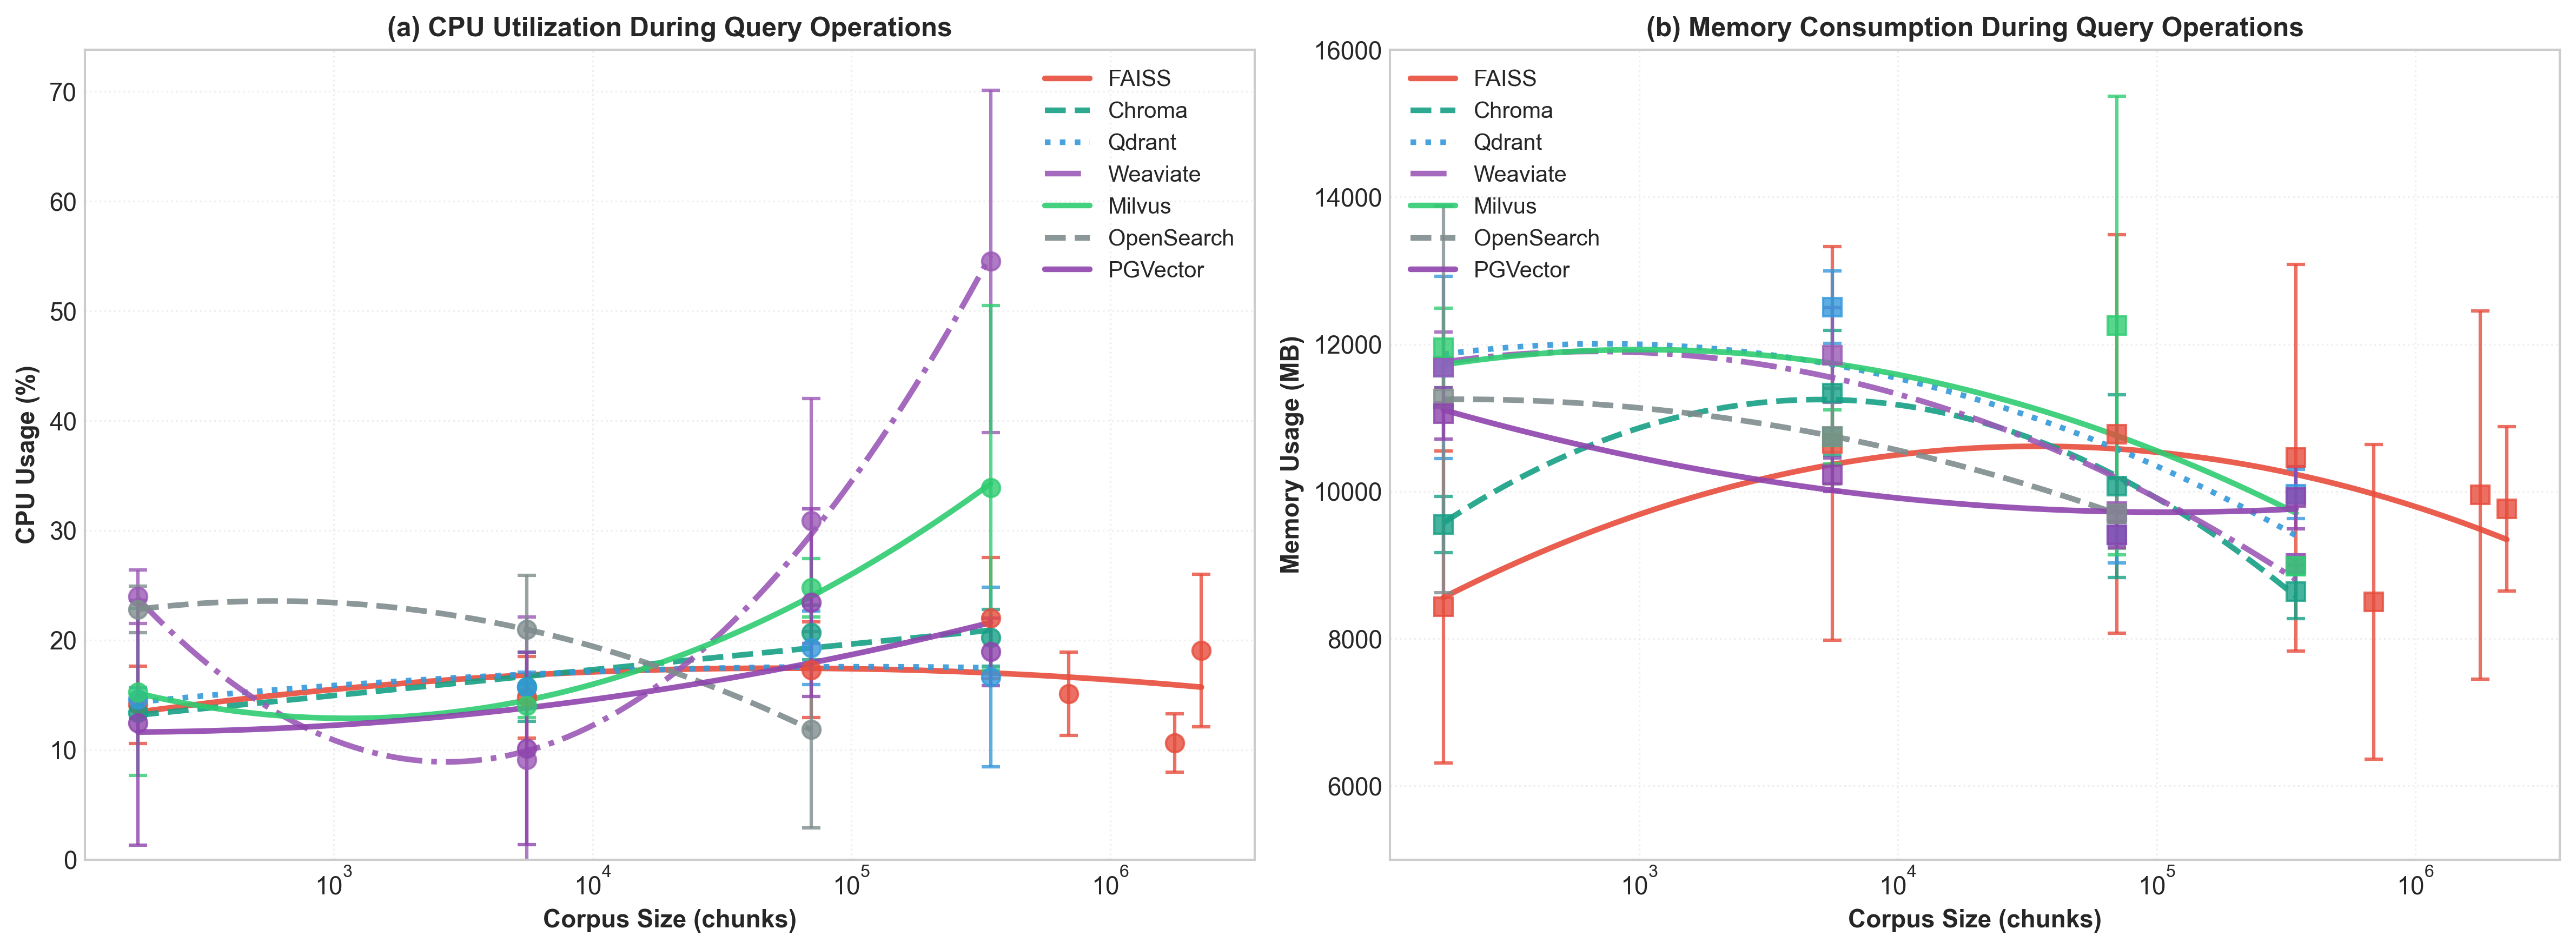
\includegraphics[width=\linewidth]{Resource_Utilization_CPU_Memory.png}
    \caption{CPU and memory utilization during query execution across all evaluated vector databases}
    \label{fig:resource_utilization_cpu_memory}
\end{figure}
\textbf{CPU Utilization:}
Figure~\ref{fig:resource_utilization_cpu_memory}(a) shows that average CPU utilization during query execution ranges from 16-25\%, with no direct correlation between CPU usage and performance. Chroma utilizes the highest CPU (25\%) while delivering the fastest queries (6-8~ms), whereas OpenSearch exhibits the lowest CPU utilization (16\%) but the highest latency (35-60~ms). Higher CPU utilization reflects efficient algorithmic intensity rather than overhead.

\textbf{Memory Footprint:}
As shown in Figure~\ref{fig:resource_utilization_cpu_memory}(b), memory usage remains remarkably consistent at \textbf{12-16~GB} across all databases during query execution (175 to 50k chunks). PGVector is the most memory-efficient (9.9~GB), while OpenSearch exhibits the highest footprint (15.5~GB). Memory does not scale dramatically with corpus size, indicating efficient HNSW graph representations. Typical HNSW overhead is 2-3× per vector.

This predictable footprint constrains single-node deployments: 16GB RAM supports approximately 1-2M chunks for HNSW and $>$5M chunks for FAISS flat indexes. OpenSearch's low CPU utilization combined with high latency suggests architectural bottlenecks (e.g., I/O serialization, JNI boundaries, and Lucene segment management) rather than computational inefficiency.

\medskip
\noindent\emph{Note: OpenSearch is omitted from the resource utilization plots in Figure~\ref{fig:resource_utilization_cpu_memory} because valid CPU utilization data were available for only one of the three evaluated corpus sizes. The plotting procedure requires a minimum of three data points to generate trend lines and therefore OpenSearch could not be included.}

\subsection{Retrieval Quality Paradox}
\label{sec:quality_paradox}
\begin{table}[h]
\small
\centering
\caption{Similarity Scores Reveal U-Shaped Quality Curve Across Scales (N=10)}
\begin{tabular}{lccc}
\toprule
\textbf{Corpus Scale} & \textbf{Chunks} & \textbf{Avg Similarity} & \textbf{Change from 1k} \\
\midrule
Baseline & 175 & 0.688 ± 0.002 & +37.6\% \\
\textbf{Quality Valley} & 1,000 & \textbf{0.500 ± 0.003} & baseline (worst) \\
Recovery Phase & 10,000 & 0.571 ± 0.002 & +14.1\% \\
\textbf{Peak Recovery} & 50,000 & \textbf{0.638 ± 0.002} & \textbf{+27.5\%} \\
Saturation Begins & 100,000 & 0.588 ± 0.003 & +17.6\% \\
\textbf{Plateau Region} & 250k-1M & 0.595-0.597 & +19.4\% (saturates) \\
\bottomrule
\multicolumn{4}{l}{\small *N=10 runs; outliers removed prior to similarity aggregation.}
\end{tabular}
\label{tab:quality}
\end{table}

Table~\ref{tab:quality} details the similarity scores across corpus scales. Quality follows counterintuitive U-shaped curve. \textbf{Worst retrieval quality occurs at 1k chunks} (0.500 similarity-27\% lower than baseline). From 1k to 50k, quality recovers \textbf{27.5\%}, nearly reaching baseline performance. Beyond 250k chunks, similarity stabilizes at $~59.7\%$ (FAISS) / ~64\% (HNSW), indicating semantic saturation and embedding model resolution ceiling.

\textbf{Mechanism:} HNSW graph maturation drives quality recovery:
\begin{itemize}
    \item 1k-node graphs: Sparse hierarchical structure (2-3 layers) with poor long-range connectivity
    \item 50k-node graphs: Mature structure (6-7 layers) with rich navigation enabling efficient multi-hop traversal
    \item Semantic space coverage: Larger corpora provide denser embedding space sampling, reducing boundary effects
\end{itemize}
\textbf{Cross-Database Consistency:} All HNSW-based databases return \textbf{virtually identical similarity scores} (variance $<0.0001$):
\begin{itemize}
    \item Chroma, PGVector, Qdrant, Weaviate, Milvus, OpenSearch: 0.638145 (50k corpus, k=3)
    \item FAISS (L2 distance): 0.582615 (8.7\% lower due to metric difference, not quality)
\end{itemize}

Critical implication: Retrieval quality is architecture-invariant across HNSW implementations. Selection should prioritize \textbf{performance, features and consistency}--not quality differences.

\textbf{Production Guidance:} Deploy minimum 10k chunks to avoid quality valley. Quality gains saturate at 250-500k chunks per shard-use horizontal sharding beyond this point rather than expanding single-shard corpus.

% ============================================================
% 4. DISCUSSION 
% ============================================================
\section{Discussion}
\label{sec: discussion}

\subsection{Architectural Insights}

\textbf{Embedded vs Client-Server Architecture:}

\textbf{Embedded (Chroma, FAISS):}
\begin{itemize}
    \item Advantages: Lower latency (7.7-8.4~ms vs 15-30~ms), higher throughput (141 QPS vs 30-70 QPS), no network serialization overhead
    \item Disadvantages: Single-process bottleneck, no horizontal scaling, no multi-tenancy, resource contention in shared environments
    \item Use when: Latency-critical single-tenant applications with $<$10~ms SLA and $<$100k documents
\end{itemize}

\textbf{Client-Server (Qdrant, Weaviate, Milvus, OpenSearch, PGVector):}
\begin{itemize}
    \item Advantages: Horizontal scaling, multi-tenancy with process isolation, production features (authentication, monitoring, persistence), ACID guarantees (PGVector)
    \item Disadvantages: Network overhead (2-4× latency penalty), serialization cost, operational complexity
    \item Use when: Scalable multi-tenant platforms with distributed deployment are feature requirements
\end{itemize}

\textbf{Flat vs HNSW Index Trade-offs:}

FAISS (flat index) achieves O(n) query time theoretically but O(n$^{0.48}$) practically through SIMD optimizations. HNSW achieves O(log N) at cost of 2-3× memory overhead. Crossover analysis:
\begin{itemize}
    \item $<$10k chunks: Comparable performance (FAISS 10-12~ms, Chroma 6-9~ms)
    \item 10k-100k chunks: HNSW advantage grows (FAISS 20-30~ms, Chroma 7-8~ms)
    \item $>$1M single-node: FAISS only proven option (HNSW hits 1-2M memory ceiling at 16GB)
\end{itemize}

FAISS excels in large-scale batch processing where absolute best latency unnecessary; HNSW dominates when sub-20~ms latency required at medium scale ($<$500k chunks).

\textbf{The OpenSearch Problem:}

OpenSearch demonstrates poor performance across every metric: 35-60~ms latency (highest), 17-29 QPS (lowest), and scaling failures beyond 345k chunks. Even after outlier removal improving CV from 93\% to 0.4\%, fundamental performance gaps persist.

\textbf{Root cause:} OpenSearch is fundamentally a full-text search engine (Lucene-based) with vector search added as a plugin. This architectural mismatch creates multiple bottlenecks:

\begin{enumerate}
    \item Storage inefficiency: Lucene segments optimized for inverted indexes, not dense vector layouts
    \item JVM overhead: Garbage collection pauses create unpredictable latency variance
    \item JNI bottleneck: Vector operations call native libraries via expensive Java Native Interface boundaries
    \item Coordination overhead: Elasticsearch cluster management interferes with vector query execution
\end{enumerate}

Recommendation: \textbf{Avoid OpenSearch for vector-first workloads.} Only acceptable for existing Elasticsearch deployments adding small-scale auxiliary vector search ($<$10k vectors, $<$5\% of queries) where ecosystem integration outweighs poor performance.

\subsection{Use-Case Recommendations and Decision Framework}
\label{sec:use_cases}

\begin{table}[h]
\small
\centering
\caption{Database Selection by Primary Requirement and Scale}
\begin{tabular}{lll}
\toprule
\textbf{Use Case} & \textbf{Recommended DB} & \textbf{Key Metrics} \\
\midrule
Real-time RAG ($<$10~ms) & Chroma & 7.7-8.4~ms, 141~QPS, CV=2.3\% \\
PostgreSQL Stack & PGVector & 9.9~ms, 101~QPS, ACID, CV=1.4\% \\
Large-scale ($>$100k chunks) & FAISS & 2.2M proven, CV=2.5\%, 90+ QPS \\
Enterprise Features & Qdrant & 28~ms, persistence, filtering, CV=1.0\% (post-clean) \\
Cost Optimization ($>$800k) & FAISS & 3.75× cheaper than HNSW \\
\bottomrule
\end{tabular}
\label{tab:usecases}
\end{table}

Table~\ref{tab:usecases} maps primary requirements to recommended databases.

\textbf{Selection Criteria:}

\textbf{Latency Requirement $<$10~ms:} Chroma dominates (6-8~ms stable) for embedded use cases; PGVector excellent (9.9~ms) for PostgreSQL ecosystem integration. Both maintain $>$100 QPS.

\textbf{Scale $>$100k Chunks:} FAISS only proven single-node option to 2.2M chunks. Client-server HNSW systems (Qdrant, Weaviate) untested beyond 100k; recommend for distributed deployments only.

\textbf{Consistency Critical:} PGVector (CV=1.4\%) and FAISS (CV=2.5\%) enable tight SLAs with minimal over-provisioning. After outlier removal, Qdrant (CV=1.0\%) and Weaviate (CV=0.8\%) also achieve excellent consistency. Treat consistency as first-class feature driving TCO.

\textbf{PostgreSQL Integration:} PGVector (second-best performance: 9.9~ms, 101~QPS) leverages existing SQL infrastructure, ACID transactions and familiar PostgreSQL ecosystem. Overhead justified when PostgreSQL already deployed for relational data.

\textbf{Production Guidelines:}
\label{sec:deployment_guidance}
\begin{itemize}
    \item Deploy HNSW with corpus $\geq$50k chunks for optimal warm-up maturation
    \item Minimum 10k chunks to avoid quality valley (0.500 at 1k → 0.638 at 50k)
    \item Shard at 250-500k chunks-quality and HNSW graph optimality saturate beyond
    \item Plan memory: 16GB supports 1-2M chunks (HNSW), 5M+ chunks (FAISS)
    \item Factor CV into capacity planning: post-outlier-removal CV reflects steady-state performance
\end{itemize}

% ============================================================
% 5. CONCLUSION 
% ============================================================
\section{Conclusion}
\label{sec: conclusion}

This N=10 statistical benchmark provides the first quantitative guidance for vector database selection across four orders of magnitude (175 to 2.2M chunks), with rigorous outlier detection revealing the critical cold-start phenomenon. Our findings reveal distinct performance classes and architectural trade-offs:

\textbf{Performance Leaders:}
\begin{itemize}
    \item Speed Champion: Chroma (\textbf{7.7-8.4~ms}, 141~QPS, $\alpha=0.02$ constant-time)
    \item Scale Champion: FAISS (proven to \textbf{2.2M chunks}, $\alpha=0.48$ sub-linear, CV=2.5\%)
    \item Production Balanced: Qdrant (28~ms, 60-70 QPS, features, CV=1.0\% post-clean)
    \item PostgreSQL Excellence: PGVector (9.9~ms, 101~QPS, ACID, CV=1.4\%)
\end{itemize}

\textbf{Novel Discoveries:}
\begin{enumerate}
    \item Cold-start phenomenon: Extended N=10 sampling reveals inflated variance in small-sample benchmarks. Qdrant 123\% → 1.0\% CV (122× improvement), Weaviate 107\% → 0.8\% (133× improvement), OpenSearch 93\% → 0.4\% (232× improvement) after outlier removal.
    \item HNSW warm-up phenomenon: \textbf{74\% latency reduction} from 1k to 50k chunks due to graph maturation
    \item Retrieval quality paradox: U-shaped curve with worst quality at 1k chunks and \textbf{27.5\% improvement by 50k}
    \item Consistency matters: Outlier removal reveals that apparent poor consistency reflects transient initialization, not algorithmic instability
\end{enumerate}

\textbf{Architectural Insights:}
\begin{itemize}
    \item Embedded architecture delivers 2-4× lower latency than client-server but lacks scaling
    \item Flat indexes (FAISS) outperform HNSW at $>$1M single-node scale
    \item OpenSearch architectural mismatch (Lucene-based) creates fundamental performance limitations
\end{itemize}

% ============================================================
% 6. LIMITATIONS
% ============================================================

\section{Limitations}
\label{sec:limitations}

While this study provides rigorous statistical characterization of vector database performance at single-node scale, several limitations should be noted:

\begin{itemize}
    \item \textbf{Sample Size Variation:}  
    All databases were tested with $N=10$ runs and formal outlier removal. 

    \item \textbf{OpenSearch Limited Scale Testing:}  
    OpenSearch experiments were restricted to corpus sizes up to 10k chunks due to timeout failures at larger scales. This limitation prevents characterization of OpenSearch scaling behavior beyond 100k chunks.

    \item \textbf{Conservative Outlier Removal:}  
    The modified Z-score threshold ($|Z| > 3.5$) was deliberately conservative to avoid over-cleaning legitimate performance variation. As a result, some residual cold-start artifacts may remain, particularly for high-variance systems.

    \item \textbf{Single-Node Evaluation:}  
    All experiments were conducted on a single compute node with 16GB RAM and an Apple Silicon CPU. Distributed scaling behavior, GPU-accelerated variants, and cross-node communication overhead remain uncharacterized.

    \item \textbf{Fixed Workload Profile:}  
    The evaluation used a fixed corpus of climate science documents with 512-character chunks. The test queries distribution  may not reflect real-world workloads with diverse semantic patterns or adversarial queries.

    \item \textbf{Index Parameter Standardization:}  
    All databases were evaluated using production-recommended default settings. Extensive parameter tuning (e.g., HNSW $M$, $ef\_construction$, $ef\_search$) could substantially shift performance characteristics.

   
\end{itemize}

% ============================================================
% 7. Future Work
% ============================================================

\section{Future Work}
~\label{sec: future} 
This study establishes statistically rigorous performance baselines for vector databases under single-node, CPU-based workloads. Several important research directions remain open:

\begin{itemize}
  \item \textbf{Distributed Scaling}: Extend benchmarks to multi-node deployments for Qdrant, Milvus and Weaviate to evaluate horizontal scalability, network overhead and shard-level consistency.
  
  \item \textbf{GPU Acceleration}: Benchmark FAISS and HNSW variants with GPU support to quantify latency, throughput and cost-efficiency improvements at multi-million scale.
  
  \item \textbf{Larger-Scale Corpora}: Evaluate performance beyond 2.2M chunks (10M+ vectors) to characterize memory ceilings, index degradation and sharding strategies in production environments.
  
  \item \textbf{Hybrid Search Workloads}: Measure combined keyword + vector search performance to assess real-world RAG and enterprise search scenarios.
  
  \item \textbf{Concurrent Read/Write Patterns}: Analyze query latency and consistency under mixed ingestion and retrieval workloads to model real-time update behavior.
  
  \item \textbf{Index and Parameter Tuning}: Study IVF, PQ and HNSW parameter trade-offs (e.g., \texttt{ef\_search}, \texttt{M}) to map accuracy-latency-memory frontiers.
  
  \item \textbf{Expanded Quality Metrics}: Incorporate IR-based evaluation metrics such as Recall@K, NDCG and MRR with document-level ground truth annotations.
\end{itemize}


% ============================================================
% 8. Appendix 
% ============================================================
\section{Appendix: Test Query Construction and Semantic Relevance Validation}
\label{sec: appendix}

\subsection{Query Construction}
The evaluation queries were manually constructed to ensure semantic alignment with the corpus domain and to support consistent cross-database evaluation. Query design followed three criteria:

\begin{enumerate}
\item \textbf{Domain Coverage}: Queries span multiple subdomains of climate science, including atmospheric processes, cryosphere dynamics, ocean systems, climate modeling, and feedback mechanisms.
\item \textbf{Corpus Relevance}: Each query was verified to correspond to multiple relevant passages within the corpus, avoiding out-of-domain or sparsely matched queries.
\item \textbf{Complexity Variation}: Queries range from single-concept factual questions to multi-concept explanatory queries.
\end{enumerate}

The final query set consists of the following:

\begin{enumerate}
\item What are the main drivers of climate change?
\item How do greenhouse gases affect global temperatures?
\item What is the role of carbon dioxide in climate warming?
\item How do ice cores help us understand past climate?
\item What are the effects of deforestation on climate?
\item How does ocean acidification relate to CO$_2$ levels?
\item What is the impact of melting glaciers on sea levels?
\item How do climate models predict future warming?
\item What are the feedback loops in the climate system?
\item How does solar radiation influence Earth's climate?
\end{enumerate}

The query set and corresponding corpus segments are publicly available for reproducibility.\footnote{https://github.com/Kwaai-AI-Lab/vector\_dbs\_benchmarking/blob/main/Data/test\_corpus/test\_cases.json}

\subsection{Semantic Relevance Validation}

Semantic relevance between queries and corpus content was established using a two-stage validation procedure:

\begin{enumerate}
\item \textbf{Corpus Alignment}: The corpus was curated exclusively from climate-science-focused documents, ensuring topical alignment with the query domain.
\item \textbf{Embedding-Space Verification}: Queries were embedded using the same embedding model employed for database indexing. Candidate corpus chunks were retrieved using cosine similarity, and manual inspection confirmed semantic alignment between queries and the highest-ranked chunks. 
\end{enumerate}

This procedure ensures that each query exhibits meaningful semantic overlap with the corpus without relying on external relevance labels.

\subsection{Retrieval Quality Metric and Limitations}

Retrieval quality is quantified using cosine similarity between query embeddings and retrieved chunk embeddings. This metric provides a continuous signal suitable for relative comparison across vector databases when evaluated under identical query, corpus, and embedding configurations.

However, cosine similarity does not yield absolute retrieval effectiveness measures. Standard Information Retrieval (IR) metrics, such as Precision@K, Recall@K, NDCG, and MRR, require labeled relevance judgments and larger evaluation sets. Future work should incorporate established benchmark datasets (e.g., MS MARCO, Natural Questions) to enable comprehensive evaluation using standard IR metrics.
% ============================================================
% 8. References
% ============================================================
\stepcounter{section}
\bibliographystyle{IEEEtran}
\bibliography{references}

\end{document}
